Dynamic and non-hierarchic mesh networks are a type of wireless network architecture that allows for the creation of ad hoc networks in which nodes can communicate with each other without the need for a central coordinating device. This type of network is characterized by its ability to self-organize and dynamically adapt to both changes in the environment and in the overall network topology. As presented in Section~\ref{sec:background-wireless-mesh-networks}, one of the key features that materializes the concept of dynamic and non-hierarchic mesh networks is the existence and implementation of lower-layer routing protocols to facilitate the peer-to-peer communication between the nodes.

Mesh networks, as expected, rely first on the physical layer, according to the standards of computer networking, which is responsible for transmitting raw bit stream data over the physical medium, copper wire, optical fibre, or wireless frequencies, for example. This layer defines the physical characteristics of the data transmission, such as voltage levels, data rates, and the physical connectors and media used for communication. Its main function is to provide a reliable and efficient transmission of bits between devices, without any regard made to the higher-layer protocols and their associated data. The physical layer is responsible for encoding and decoding data into a format that can be transmitted over the network, while also detecting and correcting errors that occur during transmission \cite{peterson2007computer}. It also defines the substrate physical topology of the network, which describes the arrangement of the physical components such as devices, cables, and other network equipment, as depicted in Figure~\ref{fig:proof-of-location-overview-pol-mesh}. To then enable efficient and coordinated communication, there is a need for routing protocols that determine the best path for data packets to travel through.

\begin{figure}[h!]
    \begin{center}
    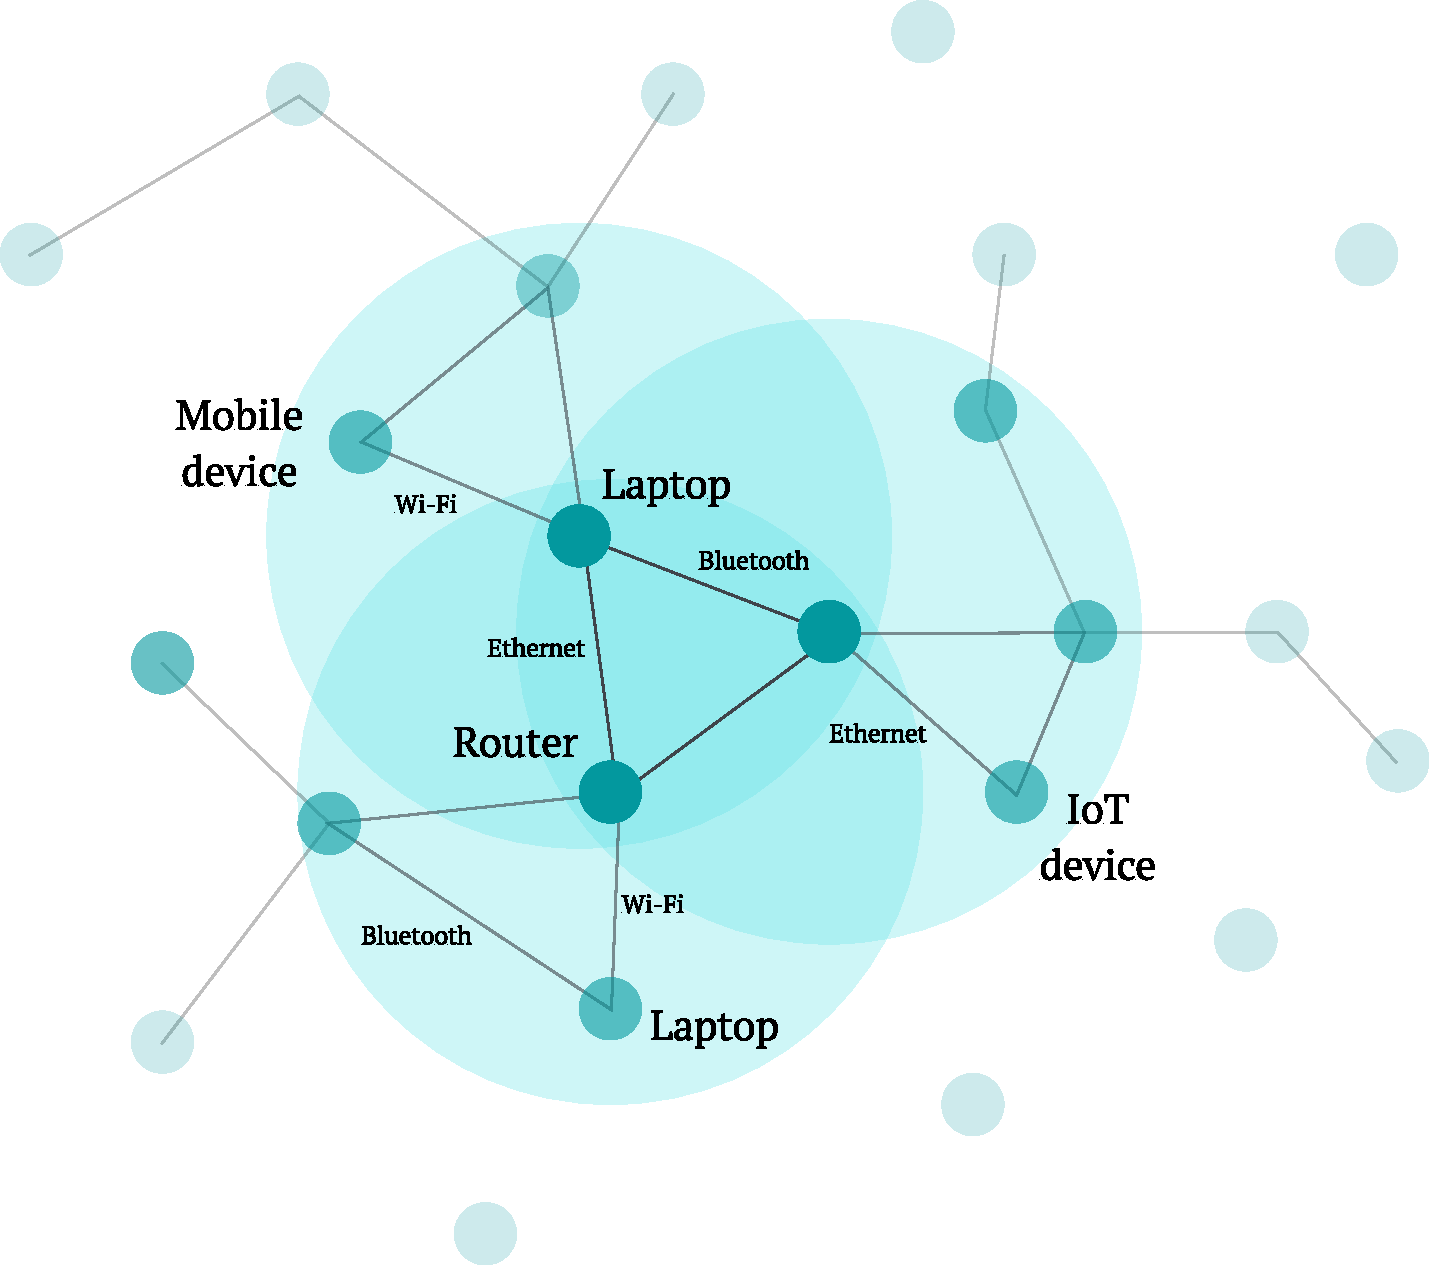
\includegraphics[width=0.65\textwidth]{overview-pol-mesh.pdf}
    \caption{The heterogeneity of a Mesh Network and the substrate diversity of its physical topology~\textemdash~the devices, their connections, and their physical arrangements.}
    \label{fig:proof-of-location-overview-pol-mesh}
    \end{center}
\end{figure}

These routing protocols are expected to operate, not at the network layer, but instead at the data link layer, which is responsible for handling the transmission of data frames over the physical layer. Their main goal is to determine the best path for data frames to travel, based on metrics gathered from lower-level physical information, as, for instance, signal strength and link stability metrics \cite{misra2009guide}. These protocols can support neighbourhood discovery and the ranking of neighbours \cite{batman-adv-v}, and thus potentially enable the processes of zone establishment and zone affinity management, as illustrated in Figure~\ref{fig:proof-of-location-overview-pol-zone-establishment}. Neighbourhood discovery is the process of physically discovering neighbouring nodes within the mesh network \cite{open-mesh-ogmv2}. Neighbour ranking is the process of determining the quality and reliability of each neighbouring link \cite{seither2011routing}. By measuring, understanding, and ranking the quality and reliability of the data links, and by instructing nodes to independently calculate their best next-hops, a routing protocol can establish neighbourhoods and determine the affinity of nodes within these coverage localities. This information can be primarily used to optimize communication paths, reduce congestion, and increase the overall efficiency of the network.

\begin{figure}[h!]
    \begin{center}
    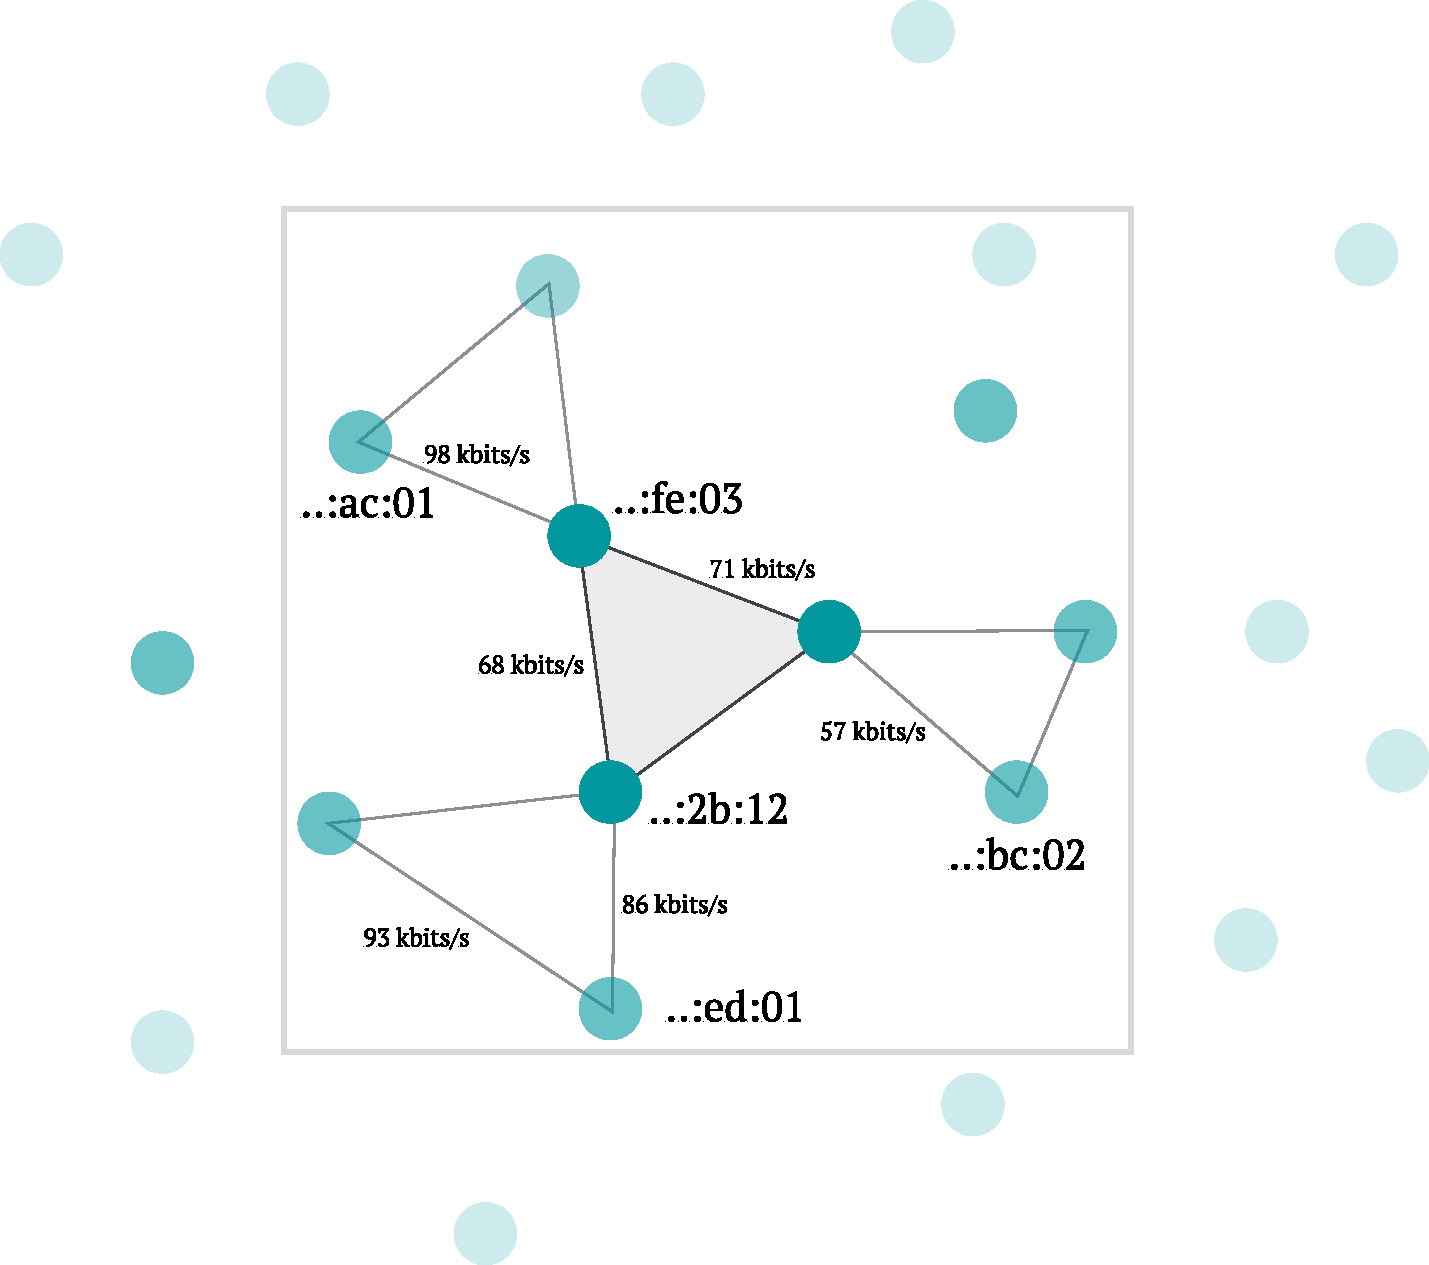
\includegraphics[width=0.7\textwidth]{overview-pol-zone-establishment.pdf}
    \caption{The routing protocol's neighbourhood discovery and ranking processes, using the MAC sublayer and link quality metrics, to enable the establishment of zones within the mesh network.}
    \label{fig:proof-of-location-overview-pol-zone-establishment}
    \end{center}
\end{figure}

The second usage of such accomplishment is to finally enable the targetted establishment of zones within the mesh network. Zones can be viewed as strongly connected sets of neighbours, that, in consequence, are one-hop away from each other. This process of zone establishment is facilitated by the routing protocol, but not strictly enforced, as the protocol solely enables the discovery of potential neighbours and the ranking of their links. The final decision of which nodes are to be grouped together into a zone is left to the nodes themselves, which can then use this information to establish their own zone affinity. Zone affinity is the process of determining the likelihood of nodes communicating and establishing zones with other nodes. The motivation may also be extrinsic to the process of zone discovery or establishment. An identity management protocol, for instance, can be used to determine the zone affinity of nodes, based on their identity and their individual wishes to communicate with other nodes. Incentives of higher degree can be used to motivate nodes to communicate, to establish zones with other relatively specific sets of nodes, and hence to collaborate in the next step of providing zone-relative location services. 
\TODO{Above is too abstract, need example...}
The FOAM protocol, for example, envisions the reliance on token-curated registries to provide a decentralized identity management. It may also rely on crypto-economic incentives to motivate nodes to collaborate and, together, establish and maintain coverage zones, for the higher purpose of providing \pol{} capabilities \cite{foam-white-paper}. This thesis' main focus, with regard to the \poc{} implementation, is abstracted from the whole process of zone establishment and zone affinity management, and assumes that a zone has been already agreed to be established by some out-of-band process. Nonetheless, these aspects are still to be identified for future work, as they are essential for the overall success of the protocol.

After the establishment of operational zones and the affinity filtering potentially happening at the data link layer, the typical Internet Protocol or TCP/IP suite can be used to enable end-to-end data communication for application-specific purposes. The TCP/IP suite consists of a set of protocols that operate at the network and transport layers, providing end-to-end communication services for applications running on different nodes \cite{peterson2007computer}. At the network layer, the Internet Protocol (IP) is used to route data packets within and between the zones, based on their IP addresses. IP is a connectionless protocol that operates independently of the underlying physical and data link layers, allowing it to be used with a variety of network technologies. At the transport layer, protocols such as TCP and UDP can be used to enable end-to-end data communication between application instances. TCP is a reliable, connection-oriented protocol that provides features such as flow control, error detection, and congestion avoidance to ensure that data is transmitted reliably and efficiently between applications. UDP, on the other hand, is a connectionless protocol that provides a lightweight alternative to TCP, suitable for applications that require low-latency communication or do not require reliability guarantees at the transport layer \cite{peterson2007computer}. The choice between the two may be based on the application requirements, the network topology, and the available resources, but the overall conclusion is that, after enabling network layer capabilities, any typical Internet service can be provided to the end-users, sustained by the underlying mesh network. Additionally, as pictured in Figure~\ref{fig:proof-of-location-overview-pol-zone-affinity}, by subnetting and assigning a unique range of IP addresses to each zone, nodes can communicate with each other, in the same zone, and with nodes in other zones using IP-based protocols. Subnetting can also provide a range of benefits, such as improved security, better network management, and more efficient address assignment and usage \cite{peterson2007computer}.

\begin{figure}[h!]
    \begin{center}
    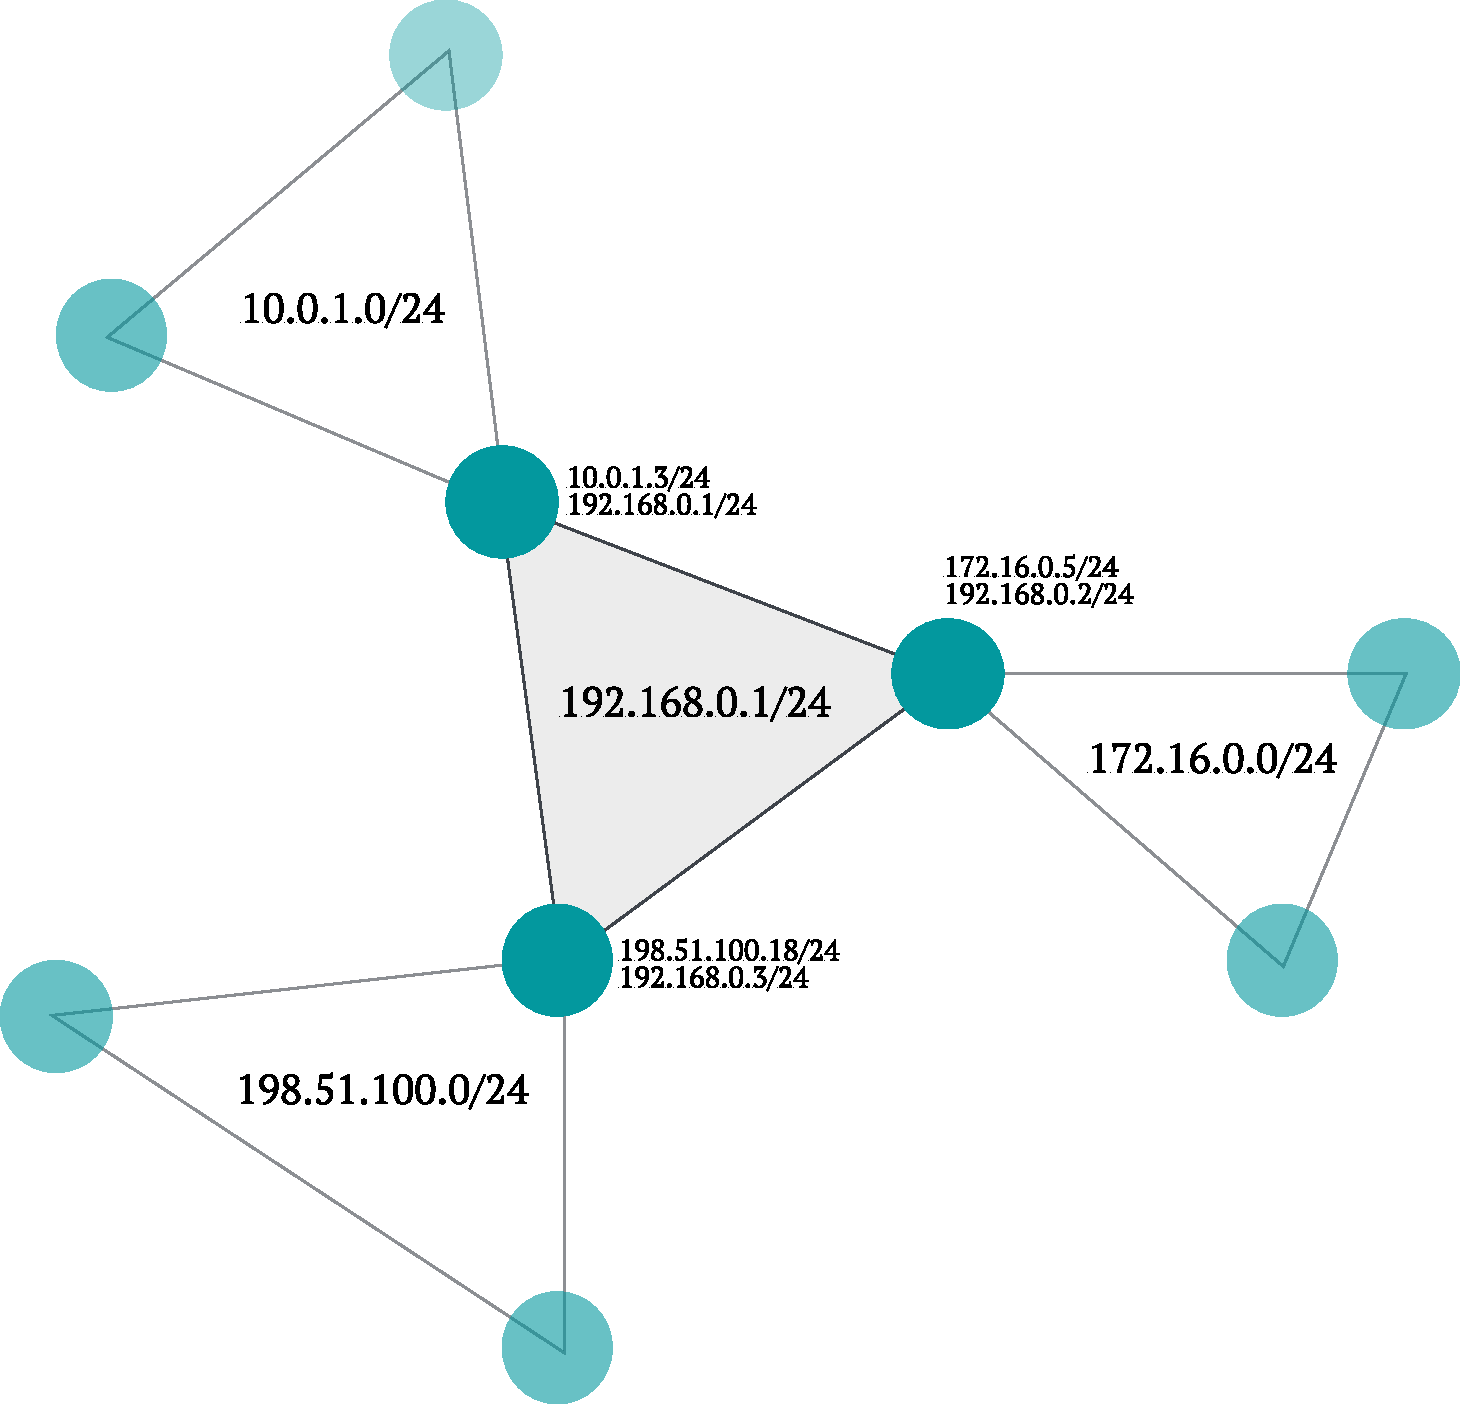
\includegraphics[width=0.6\textwidth]{overview-pol-zone-affinity.pdf}
    \caption{Subnetting and IP-based communication between nodes, within and between zones, after the establishment of their respective zone affinities.}
    \label{fig:proof-of-location-overview-pol-zone-affinity}
    \end{center}
\end{figure}

The following section presents the next step towards guaranteeing the infrastructural basis of the proposed \pol{} protocol, detailing not only the need for zone-relative clock synchronization, but also the steps taken to eventually achieve spatio-temporal soundness. It ultimately assumes that the physical, data link, network, and transport layer capabilities have been already established, and that the nodes are able to communicate with each other using the TCP/IP suite and related protocols, on top of the underlying mesh network infrastructure. The verification or enforcement of the usage of short range communication means is still to be researched, as a key aspect to the protocol's foundational security, and soundness guarantees.